\documentclass[12pt]{article}

\title{Initial conditions}
\author{Jan Medlock et al.}

\usepackage{microtype}
\usepackage{tikz}
\usepackage{hyperref}
\hypersetup{breaklinks}
\hypersetup{pdfborder=0 0 0}
\usepackage{natbib}
\usepackage{hypernat}
\usepackage{amsmath}
\renewcommand{\vec}[1]{\mathbf{#1}}
\newcommand{\mat}[1]{\mathbf{#1}}
\DeclareMathOperator{\Prob}{Prob}
\DeclareMathOperator{\diag}{diag}
\newcommand{\md}{\mathrm{d}}
\newcommand{\me}{\mathrm{e}}
\newcommand{\mT}{\mathrm{T}}
\setcounter{MaxMatrixCols}{12}


\begin{document}

\maketitle

We will find the equilibrium probability as a function of age of being
in each model compartment (\autoref{model_diagram}), i.e.
\begin{equation}
  P_X(a) = \Prob\{\text{in compartment $X$ at age $a$}|\text{alive at
    age $a$}\},
\end{equation}
for $X \in \{\mathrm{M}, \mathrm{S}, \mathrm{E}, \mathrm{I},
\mathrm{C}, \mathrm{R}, \mathrm{L}\}$ and $a \geq 0$.
We will assume that
\begin{itemize}
\item the infection hazard is constant, and
\item all calves are born with maternal immunity.
\end{itemize}

\begin{figure}
  \begin{center}
    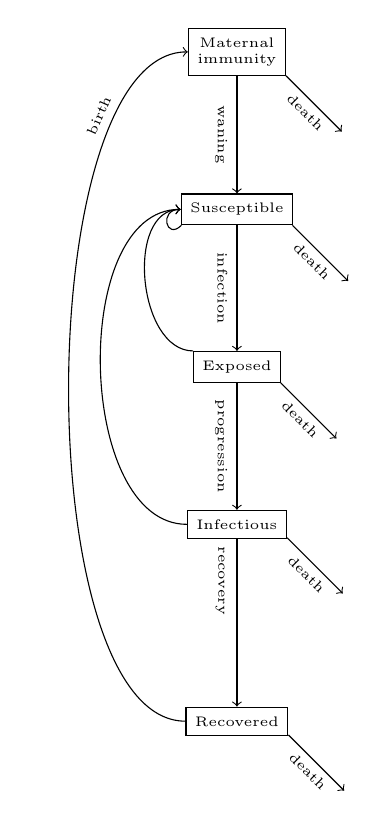
\begin{tikzpicture}[compartment/.style = {rectangle, draw}, font=\fontsize{5pt}{6}\selectfont]
  % Compartments.
  \node at (0, 11) [compartment, align=center, name=MaternalImmunity] {Maternal\\immunity};
  \node at (0, 9) [compartment, name=Susceptible] {Susceptible};
  \node at (0, 7) [compartment, name=Exposed] {Exposed};
  \node at (0, 5) [compartment, name=Infectious] {Infectious};
  \node at (0, 2.5) [compartment, name=Recovered] {Recovered};

  % Location for branch from Infectious to Chronic and Recovered.
  \coordinate (recovery) at (0, 3.75);

  % Infection-related processes.
  \draw [->] (MaternalImmunity)
             to node [rotate=-90, below] {waning}
             (Susceptible);
  \draw [->] (Susceptible)
             to node [rotate=-90, below] {infection}
             (Exposed);
  \draw [->] (Exposed)
             to node [rotate=-90, below] {progression}
             (Infectious);
  \draw [  ] (Infectious)
             to node [rotate=-90, below, yshift=-1pt] {recovery}
             (recovery);
  \draw [->] (recovery)
             to node [] {}
             (Recovered.90);

  % Births
  \draw [->] (Susceptible.196)
             to [out=225, in=180, looseness=3.5] node [] {}
             (Susceptible.180);
  \draw [->] (Exposed.160)
             to [out=180, in=180] node [] {}
             (Susceptible.180);
  \draw [->] (Infectious.180)
             to [out=180, in=180, looseness=0.9] node [sloped, above, pos=0.85] {}
             (Susceptible.180);
  \draw [->] (Recovered.180)
             to [out=180, in=180, looseness=0.6] node [sloped, above, pos=0.8] {birth}
             (MaternalImmunity.180);

  % Deaths
  \draw [->] (MaternalImmunity.334)
             to node [sloped, below, yshift=1pt] {death}
             +(315: 1);
  \draw [->] (Susceptible.344)
             to node [sloped, below, yshift=1pt] {death}
             +(315: 1);
  \draw [->] (Exposed.340)
             to node [sloped, below, yshift=1pt] {death}
             +(315: 1);
  \draw [->] (Infectious.345)
             to node [sloped, below, yshift=1pt] {death}
             +(315: 1);
  \draw [->] (Recovered.345)
             to node [sloped, below, yshift=1pt] {death}
             +(315: 1);
\end{tikzpicture}

%%% Local Variables:
%%% mode: latex
%%% TeX-master: "diagram_standalone"
%%% End:

  \end{center}
  \caption{Model diagram.}
  \label{model_diagram}
\end{figure}

The compartment probabilities satisfy
\begin{equation}
  \begin{split}
    \frac{\md P_{\mathrm{M}}}{\md a}
    &= - h_{\text{waning}}(a) P_{\mathrm{M}}(a),
    \\
    \frac{\md P_{\mathrm{S}}}{\md a}
    &= h_{\text{waning}}(a) P_{\mathrm{M}}(a)
    - h_{\text{infection}} P_{\mathrm{S}}(a),
    \\
    \frac{\partial p_{\mathrm{E}}}{\partial a}
    + \frac{\partial p_{\mathrm{E}}}{\partial r}
    &= - h_{\text{progression}}(r) p_{\mathrm{E}}(a, r),
    \\
    p_{\mathrm{E}}(a, 0) &= h_{\text{infection}}
    \big(P_{\mathrm{S}}(a) + P_{\mathrm{L}}(a)\big),
    \\
    \frac{\partial p_{\mathrm{I}}}{\partial a}
    + \frac{\partial p_{\mathrm{I}}}{\partial r}
    &= - h_{\text{recovery}}(r) p_{\mathrm{I}}(a, r),
    \\
    p_{\mathrm{I}}(a, 0) &=
    \int_0^a h_{\text{progression}}(r)
    p_{\mathrm{E}}(a, r) \md r,
    \\
    \frac{\partial p_{\mathrm{C}}}{\partial a}
    + \frac{\partial p_{\mathrm{C}}}{\partial r}
    &= - h_{\text{chronic recovery}}(r) p_{\mathrm{C}}(a, r),
    \\
    p_{\mathrm{C}}(a, 0) &=
    p_{\text{chronicity}}
    \int_0^a h_{\text{recovery}}(r) p_{\mathrm{I}}(a, r) \md r,
    \\
    \frac{\md P_{\mathrm{R}}}{\md a}
    &=
    \left(1 - p_{\text{chronicity}}\right)
    \int_0^a h_{\text{recovery}}(r) p_{\mathrm{I}}(a, r) \md r
    \\ & \quad {}
    + \int_0^a h_{\text{chronic recovery}}(r) p_{\mathrm{C}}(a, r) \md r
    \\ & \quad {}
    + h_{\text{antibody gain}} P_{\mathrm{L}}(a)
    - h_{\text{antibody loss}} P_{\mathrm{R}}(a),
    \\
    \frac{\md P_{\mathrm{L}}}{\md a}
    &=
    h_{\text{antibody loss}} P_{\mathrm{R}}(a)
    - \left(h_{\text{antibody gain}} + h_{\text{infection}}\right)
    P_{\mathrm{L}}(a)
  \end{split}
\end{equation}
for $0 \leq r \leq a$,
with
\begin{equation}
  \begin{split}
    P_{\mathrm{M}}(0) &= 1,
    \\
    P_{\mathrm{S}}(0) &= 0,
    \\
    p_{\mathrm{E}}(0, 0) &= 0,
    \\
    p_{\mathrm{I}}(0, 0) &= 0,
    \\
    p_{\mathrm{C}}(0, 0) &= 0,
    \\
    P_{\mathrm{R}}(0) &= 0,
    \\
    P_{\mathrm{L}}(0) &= 0,
  \end{split}
\end{equation}
and
\begin{equation}
  P_X(a) = \int_0^a p_X(a, r) \md r,
\end{equation}
for $X \in \{\mathrm{E}, \mathrm{I}, \mathrm{C}\}$.

\section{Numerical method}

To compute the compartment probabilities, we used the Crank--Nicolson
method on characteristics and the composite trapezoid rule for the
integrals \citep{milner_1992}.  Given the age step $\Delta a$, let
$a^i = i \Delta a$ and $r^j = j \Delta a$ for $i, j \in \{0, 1, 2,
\ldots, I - 1\}$, $P_X^i \approx P_X(a^i)$, and $p_X^{i, j} \approx
p_X(a^i, r^j)$.
For each $1 \leq i \leq I - 1$ and each $1 \leq j \leq i$, the
Crank--Nicolson method on characteristics is
\begin{equation}
  \begin{split}
    P_{\mathrm{M}}^0 &= 1,
    \\
    \frac{P_{\mathrm{M}}^i - P_{\mathrm{M}}^{i - 1}}{\Delta a}
    &= - h_{\text{waning}}(a^{i - 1 / 2})
    \frac{P_{\mathrm{M}}^i + P_{\mathrm{M}}^{i - 1}}{2},
    \\
    P_{\mathrm{S}}^0 &= 0,
    \\
    \frac{P_{\mathrm{S}}^i - P_{\mathrm{S}}^{i - 1}}{\Delta a}
    &= h_{\text{waning}}(a^{i - 1 / 2})
    \frac{P_{\mathrm{M}}^i + P_{\mathrm{M}}^{i - 1}}{2}
    - h_{\text{infection}}
    \frac{P_{\mathrm{S}}^i + P_{\mathrm{S}}^{i - 1}}{2},
    \\
    p_{\mathrm{E}}^{0, 0} &= 0,
    \\
    p_{\mathrm{E}}^{i, 0} &= h_{\text{infection}}
    \left(\frac{P_{\mathrm{S}}^i + P_{\mathrm{S}}^{i - 1}}{2}
    + \frac{P_{\mathrm{L}}^i + P_{\mathrm{L}}^{i - 1}}{2}\right),
    \\
    \frac{p_{\mathrm{E}}^{i, j} - p_{\mathrm{E}}^{i - 1, j - 1}}{\Delta a}
    &= - h_{\text{progression}}(r^{j - 1 / 2})
    \frac{p_{\mathrm{E}}^{i, j} + p_{\mathrm{E}}^{i - 1, j - 1}}{2},
    \\
    p_{\mathrm{I}}^{0, 0} &= 0,
    \\
    p_{\mathrm{I}}^{i, 0} &=
    \frac{\pi^i + \pi^{i - 1}}{2},
    \\
    \frac{p_{\mathrm{I}}^{i, j} - p_{\mathrm{I}}^{i - 1, j - 1}}{\Delta a}
    &= - h_{\text{recovery}}(r^{j - 1 / 2})
    \frac{p_{\mathrm{I}}^{i, j} + p_{\mathrm{I}}^{i - 1, j - 1}}{2},
    \\
    p_{\mathrm{C}}^{0, 0} &= 0,
    \\
    p_{\mathrm{C}}^{i, 0} &= p_{\text{chronicity}}
    \frac{\rho^i + \rho^{i - 1}}{2},
    \\
    \frac{p_{\mathrm{C}}^{i, j} - p_{\mathrm{C}}^{i - 1, j - 1}}{\Delta a}
    &= - h_{\text{chronic recovery}}(r^{j - 1 / 2})
    \frac{p_{\mathrm{C}}^{i, j} + p_{\mathrm{C}}^{i - 1, j - 1}}{2},
    \\
    P_{\mathrm{R}}^0 &= 0,
    \\
    \frac{P_{\mathrm{R}}^i - P_{\mathrm{R}}^{i - 1}}{\Delta a}
    &= \big(1 - p_{\text{chronicity}}\big) \frac{\rho^i + \rho^{i - 1}}{2}
    + \frac{\chi^i + \chi^{i - 1}}{2}
    \\ & \quad {}
    - h_{\text{antibody loss}}
    \frac{P_{\mathrm{R}}^i + P_{\mathrm{R}}^{i - 1}}{2}
    + h_{\text{antibody gain}}
    \frac{P_{\mathrm{L}}^i + P_{\mathrm{L}}^{i - 1}}{2},
    \\
    P_{\mathrm{L}}^0 &= 0,
    \\
    \frac{P_{\mathrm{L}}^i - P_{\mathrm{L}}^{i - 1}}{\Delta a}
    &= h_{\text{antibody loss}}
    \frac{P_{\mathrm{R}}^i + P_{\mathrm{R}}^{i - 1}}{2}
    - h_{\text{antibody gain}}
    \frac{P_{\mathrm{L}}^i + P_{\mathrm{L}}^{i - 1}}{2},
  \end{split}
\end{equation}
where
\begin{equation}
  \begin{split}
    \pi^i &=
    \sum_{j = 0}^i T^{i, j} h_{\text{progression}}(r^j) p_{\mathrm{E}}^{i, j},
    \\
    \rho^i &=
    \sum_{j = 0}^i T^{i, j} h_{\text{recovery}}(r^j) p_{\mathrm{I}}^{i, j},
    \\
    \chi^i &=
    \sum_{j = 0}^i T^{i, j} h_{\text{chronic recovery}}(r^j) p_{\mathrm{C}}^{i, j},
  \end{split}
\end{equation}
and
\begin{equation}
  T^{i, j} =
  \begin{cases}
    \frac{\Delta a}{2} & \text{if $j = 0$ or $j = i$}, \\
    \Delta a & \text{if $1 \leq j \leq i - 1$},
  \end{cases}
\end{equation}
implements the composite trapezoid rule.
Then
\begin{equation}
  \begin{split}
    P_E^i &= \sum_{j = 0}^i T^{i, j} p_{\mathrm{E}}^{i, j},
    \\
    P_I^i &= \sum_{j = 0}^i T^{i, j} p_{\mathrm{I}}^{i, j},
    \\
    P_C^i &= \sum_{j = 0}^i T^{i, j} p_{\mathrm{C}}^{i, j}.
  \end{split}
\end{equation}

For the variables $P_X$ that only depend on age $a$,
define the vectors
\begin{equation}
  \vec{P}_X =
  \begin{pmatrix}
    P_X^0\\
    P_X^1\\
    \vdots\\
    P_X^{I - 1}
  \end{pmatrix},
\end{equation}
for $X \in \{\mathrm{M}, \mathrm{S}, \mathrm{R}, \mathrm{L}\}$.
For the variables that depend on age $a$ and residence time $r$,
define the vectors
\begin{equation}
  \vec{p}_X =
  \begin{pmatrix}
    p_X^{0, 0}\\
    p_X^{1, 0}\\
    p_X^{1, 1}\\
    p_X^{2, 0}\\
    p_X^{2, 1}\\
    p_X^{2, 2}\\
    \vdots\\
    p_X^{I - 1, 0}\\
    \vdots\\
    p_X^{I - 1, I - 1}
  \end{pmatrix},
\end{equation}
for $X \in \{\mathrm{E}, \mathrm{I}, \mathrm{C}\}$,
where the $i, j$th entry is in position
\begin{equation}
  k = \frac{i (i + 1)}{2} + j,
\end{equation}
or
\begin{equation}
  \begin{split}
    i &= \left\lfloor\frac{- 1 + \sqrt{8 k + 1}}{2}\right\rfloor,
    \\
    j &= k - \frac{i (i + 1)}{2}.
  \end{split}
\end{equation}
Then for $1 \leq i \leq I - 1$ and $1 \leq j \leq i$,
\begin{equation}
  \begin{split}
    P_{\mathrm{M}}^0 &= 1,
    \\
    \left[2 - h_{\text{waning}}(a^{i - 1 / 2}) \Delta a\right]
    P_{\mathrm{M}}^{i - 1}
    - \left[2 + h_{\text{waning}}(a^{i - 1 / 2}) \Delta a\right]
    P_{\mathrm{M}}^i
    &= 0,
  \end{split}
\end{equation}
\begin{equation}
  \begin{split}
    P_{\mathrm{S}}^0 &= 0,
    \\
    h_{\text{waning}}(a^{i - 1 / 2}) \Delta a P_{\mathrm{M}}^{i - 1}
    + h_{\text{waning}}(a^{i - 1 / 2}) \Delta a P_{\mathrm{M}}^i
    \\ {}
    + \left[2 - h_{\text{infection}} \Delta a\right]
    P_{\mathrm{S}}^{i - 1}
    - \left[2 + h_{\text{infection}} \Delta a\right]
    P_{\mathrm{S}}^i
    &= 0,
  \end{split}
\end{equation}
\begin{equation}
  \begin{split}
    P_{\mathrm{R}}^0 &= 0,
    \\
    \left[2 - h_{\text{antibody loss}} \Delta a\right]
    P_{\mathrm{R}}^{i - 1}
    - \left[2 + h_{\text{antibody loss}} \Delta a\right]
    P_{\mathrm{R}}^i
    \\ {}
    + h_{\text{antibody gain}} \Delta a P_{\mathrm{L}}^{i - 1}
    + h_{\text{antibody gain}} \Delta a P_{\mathrm{L}}^i
    \\ {}
    + \sum_{j = 0}^{i - 1}
    T^{i - 1, j} \left(1 - p_{\text{chronicity}}\right)
    h_{\text{recovery}}(r^j) \Delta a
    p_{\mathrm{I}}^{i - 1, j}
    \\ {}
    + \sum_{j = 0}^i
    T^{i, j} \left(1 - p_{\text{chronicity}}\right)
    h_{\text{recovery}}(r^j) \Delta a
    p_{\mathrm{I}}^{i, j}
    \\ {}
    + \sum_{j = 0}^{i - 1}
    T^{i - 1, j} h_{\text{chronic recovery}}(r^j) \Delta a
    p_{\mathrm{C}}^{i - 1, j}
    \\ {}
    + \sum_{j = 0}^i
    T^{i, j} h_{\text{chronic recovery}}(r^j) \Delta a
    p_{\mathrm{C}}^{i, j}
    &= 0,
  \end{split}
\end{equation}
\begin{equation}
  \begin{split}
    P_{\mathrm{L}}^0 &= 0,
    \\
    h_{\text{antibody loss}} \Delta a P_{\mathrm{R}}^{i - 1}
    + h_{\text{antibody loss}} \Delta a P_{\mathrm{R}}^i
    \\ {}
    + \left[2 - h_{\text{antibody gain}} \Delta a\right]
    P_{\mathrm{L}}^{i - 1}
    - \left[2 + h_{\text{antibody gain}} \Delta a\right]
    P_{\mathrm{L}}^i
    &= 0,
  \end{split}
\end{equation}
\begin{equation}
  \begin{split}
    p_{\mathrm{E}}^{0, 0} &= 0,
    \\
    h_{\text{infection}} P_{\mathrm{S}}^{i - 1}
    + h_{\text{infection}} P_{\mathrm{S}}^i
    + h_{\text{infection}} P_{\mathrm{L}}^{i - 1}
    + h_{\text{infection}} P_{\mathrm{L}}^i
    - 2 p_{\mathrm{E}}^{i, 0}
    &= 0,
    \\
    \left[2 - h_{\text{progression}}(r^{j - 1 / 2}) \Delta a\right]
    p_{\mathrm{E}}^{i - 1, j - 1}
    \\ {}
    - \left[2 + h_{\text{progression}}(r^{j - 1 / 2}) \Delta a\right]
    p_{\mathrm{E}}^{i, j}
    &= 0,
  \end{split}
\end{equation}
\begin{equation}
  \begin{split}
    p_{\mathrm{I}}^{0, 0} &= 0,
    \\
    \sum_{j = 0}^{i - 1}
    T^{i - 1, j} h_{\text{progression}}(r^j) p_{\mathrm{E}}^{i - 1, j}
    + \sum_{j = 0}^i
    T^{i, j} h_{\text{progression}}(r^j) p_{\mathrm{E}}^{i, j}
    - 2 p_{\mathrm{I}}^{i, 0}
    &= 0,
    \\
    \left[2 - h_{\text{recovery}}(r^{j - 1 / 2}) \Delta a\right]
    p_{\mathrm{I}}^{i - 1, j - 1}
    - \left[2 + h_{\text{recovery}}(r^{j - 1 / 2}) \Delta a\right]
    p_{\mathrm{I}}^{i, j}
    &= 0,
  \end{split}
\end{equation}
\begin{equation}
  \begin{split}
    p_{\mathrm{C}}^{0, 0} &= 0,
    \\
    \sum_{j = 0}^{i - 1}
    T^{i - 1, j} p_{\text{chronicity}} h_{\text{recovery}}(r^j)
    p_{\mathrm{I}}^{i - 1, j}
    \\ {}
    + \sum_{j = 0}^i
    T^{i, j} p_{\text{chronicity}} h_{\text{recovery}}(r^j)
    p_{\mathrm{I}}^{i, j}
    \\ {}
    - 2 p_{\mathrm{C}}^{i, 0}
    &= 0,
    \\
    \left[2 - h_{\text{chronic recovery}}(r^{j - 1 / 2}) \Delta a\right]
    p_{\mathrm{C}}^{i - 1, j - 1}
    \\ {}
    - \left[2 + h_{\text{chronic recovery}}(r^{j - 1 / 2}) \Delta a\right]
    p_{\mathrm{C}}^{i, j}
    &= 0.
  \end{split}
\end{equation}

\bibliography{journal_abbreviations,math_epi}
\bibliographystyle{jpmbib}

\end{document}
